	~
	
	~
	
	\newcommand{\NaturalElementTextFormat}[7]
	{
		\begin{minipage}{2.21cm}
			\centering
			{\textbf{#1}\hspace{1em} \underline{{#7}} \hfill {#2}\textit{{#3}}}%
			\\[0.1cm]
			{\Huge \textbf{{#5}}}
			\linebreak
			{\fontsize{9.5}{10.0}\selectfont {#6} }
			\linebreak
			{\small {#4}} 
		\end{minipage}
	}
	
	\newcommand{\KeyTextFormat}[7]
	{
		\begin{minipage}{2.21m}
			\centering
			{\textbf{#1}\hspace{1em} \underline{{#7}} \hfill {#2}\textit{{#3}}}%
			\\[0.1cm]
			{\Huge \textbf{{#5}}}
			\linebreak
			{\fontsize{9.5}{10}\selectfont {#6} }
			\linebreak
			{\small {#4}} 
		\end{minipage}
	}
	\tikzstyle{SBlock} = [fill=yellow!10]
	\tikzstyle{PBlock} = [fill=blue!10]
	\tikzstyle{DBlock} = [fill=red!10]
	\tikzstyle{FBlock} = [fill=green!10]
	
	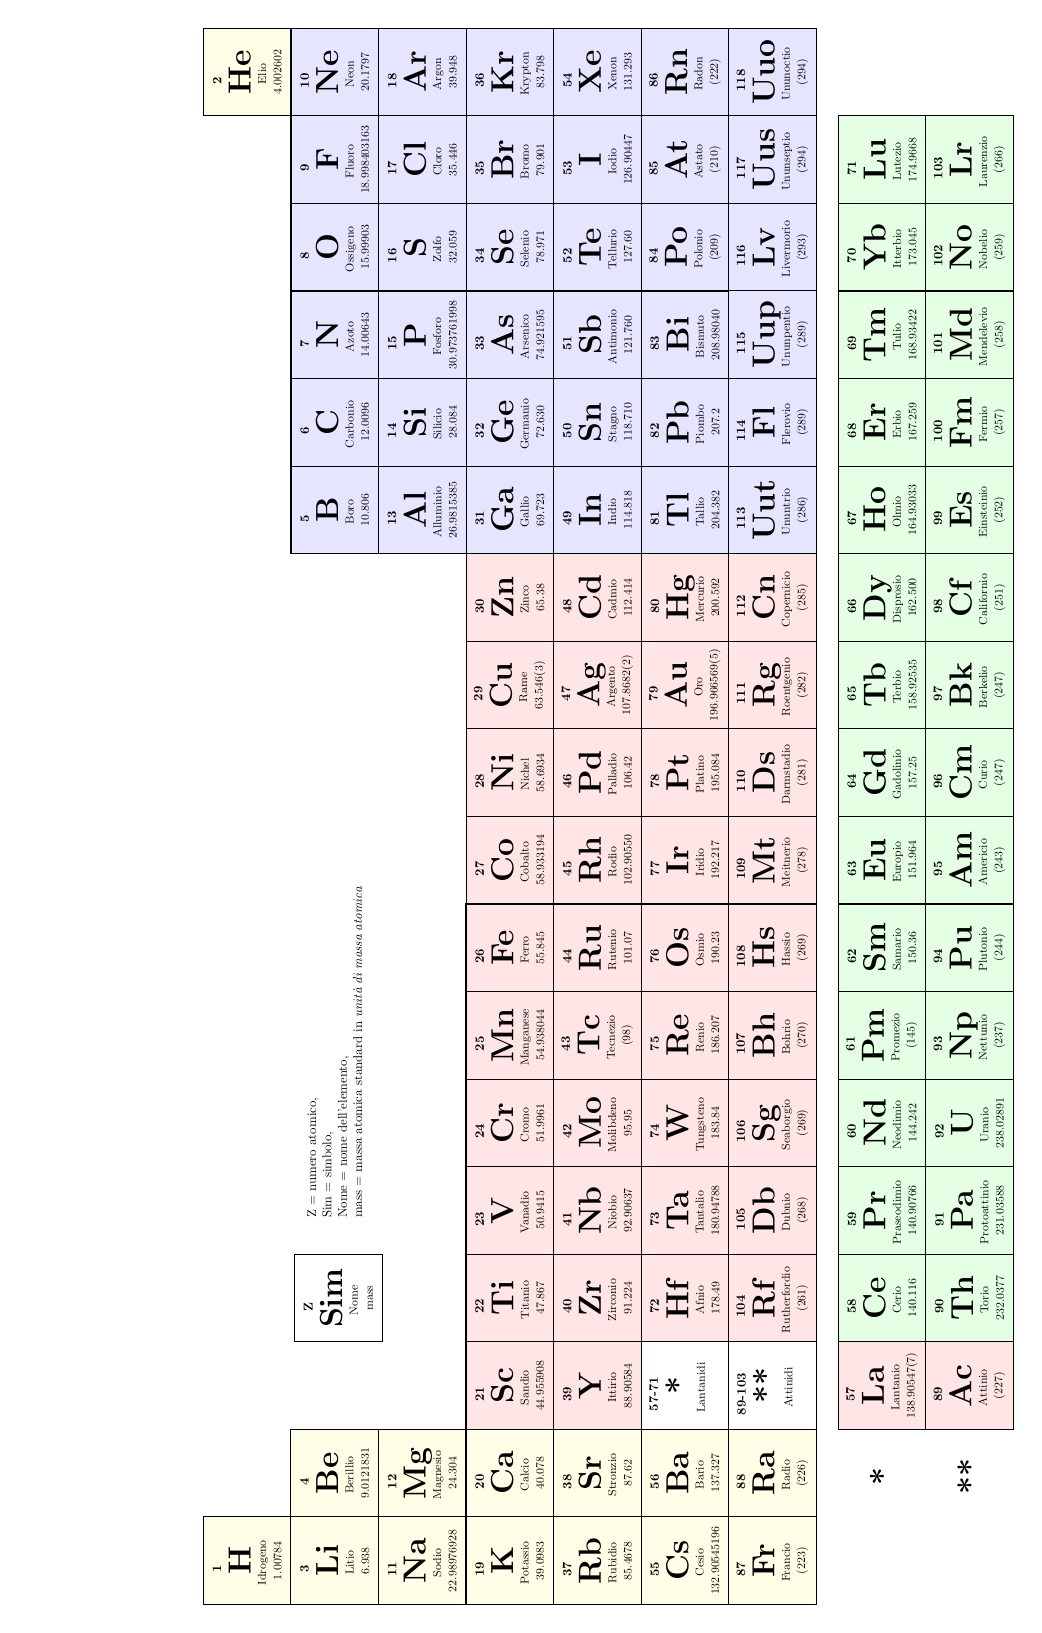
\begin{tikzpicture}[scale=0.4633, transform shape, rotate=90]
	
	\tikzstyle{KeyBox} =  [draw=black, minimum width=2.4cm, minimum height=2.4cm, node distance=2.4cm, inner sep=0pt]
	\tikzstyle{Element} = [draw=black, minimum width=2.4cm, minimum height=2.4cm, node distance=2.4cm, inner sep=0pt]
	\tikzstyle{Offsetter} = [draw=white, minimum width=2.4cm, minimum height=2.4cm, node distance=2.4cm, inner sep=0pt]
	\tikzstyle{TitleLabel} = [font={\Huge\bfseries}]
	\tikzstyle{KeysLabel} = [minimum height = 2.5cm, inner sep=0pt, text width = 10cm]
	\tikzstyle{DetailsLabel} = [minimum height = 2.5cm, node distance = 2.5cm, inner sep=0pt]
	
	%% Group 1 - IA
	\node[name=Blank1, Offsetter] {}; % this is just an invisible box that shoves the entire table downward to make it more centered
	\node[name=Blank2, below of=Blank1, Offsetter] {}; % see comment on invisible box above.
	\node[name=H,	below of=Blank2, SBlock, Element] {\NaturalElementTextFormat{1}{}{}{1.00784}{H}{Idrogeno}{}};
	\node[name=Li, 	below of=H, 	SBlock, Element] {\NaturalElementTextFormat{3}{}{}{6.938}{Li}{Litio}{}};
	\node[name=Na, 	below of=Li,	SBlock, Element] {\NaturalElementTextFormat{11}{}{}{22.98976928}{Na}{Sodio}{}};
	\node[name=K, 	below of=Na,	SBlock, Element] {\NaturalElementTextFormat{19}{}{}{39.0983}{K}{Potassio}{}};
	\node[name=Rb, 	below of=K, 	SBlock, Element] {\NaturalElementTextFormat{37}{}{}{85.4678}{Rb}{Rubidio}{}};
	\node[name=Cs, 	below of=Rb,	SBlock, Element] {\NaturalElementTextFormat{55}{}{}{132.90545196}{Cs}{Cesio}{}};
	\node[name=Fr, 	below of=Cs,	SBlock, Element] {\NaturalElementTextFormat{87}{}{}{(223)}{Fr}{Francio}{}};
	
	%% Group 2 - IIA
	\node[name=Be, right of=Li, SBlock, Element] {\NaturalElementTextFormat{4}{}{}{9.0121831}{Be}{Berillio}{}};
	\node[name=Mg, below of=Be, SBlock, Element] {\NaturalElementTextFormat{12}{}{}{24.304}{Mg}{Magnesio}{}};
	\node[name=Ca, below of=Mg, SBlock, Element] {\NaturalElementTextFormat{20}{}{}{40.078}{Ca}{Calcio}{}};
	\node[name=Sr, below of=Ca, SBlock, Element] {\NaturalElementTextFormat{38}{}{}{87.62}{Sr}{Stronzio}{}};
	\node[name=Ba, below of=Sr, SBlock, Element] {\NaturalElementTextFormat{56}{}{}{137.327}{Ba}{Bario}{}};
	\node[name=Ra, below of=Ba, SBlock, Element] {\NaturalElementTextFormat{88}{}{}{(226)}{Ra}{Radio}{}};
	
	%% Group 3 - IIIB
	\node[name=Sc, 	right of=Ca, 	DBlock,  Element] {\NaturalElementTextFormat{21}{}{}{44.955908}{Sc}{Sandio}{}};
	\node[name=Y, 	below of=Sc, 	DBlock, Element] {\NaturalElementTextFormat{39}{}{}{88.90584}{Y}{Ittirio}{}};
	\node[name=LaLu, 	below of=Y, 	Element] {\NaturalElementTextFormat{57-71}{}{}{}{*}{Lantanidi}{}};
	\node[name=AcLr, 	below of=LaLu, 	Element] {\NaturalElementTextFormat{89-103}{}{}{}{**}{Attinidi}{}};
	
	%% Group 4 - IVB
	\node[name=Ti, right of=Sc, DBlock, Element] {\NaturalElementTextFormat{22}{}{}{47.867}{Ti}{Titanio}{}};
	\node[name=Zr, below of=Ti,DBlock,  Element] {\NaturalElementTextFormat{40}{}{}{91.224}{Zr}{Zirconio}{}};
	\node[name=Hf, below of=Zr,DBlock,  Element] {\NaturalElementTextFormat{72}{}{}{178.49}{Hf}{Afnio}{}};
	\node[name=Rf, below of=Hf, DBlock, Element] {\NaturalElementTextFormat{104}{}{}{(261)}{Rf}{Rutherfordio}{}};
	
	%% Group 5 - VB
	\node[name=V, right of=Ti, DBlock, Element] {\NaturalElementTextFormat{23}{}{}{50.9415}{V}{Vanadio}{}};
	\node[name=Nb, below of=V, DBlock, Element] {\NaturalElementTextFormat{41}{}{}{92.90637}{Nb}{Niobio}{}};
	\node[name=Ta, below of=Nb, DBlock, Element] {\NaturalElementTextFormat{73}{}{}{180.94788}{Ta}{Tantalio}{}};
	\node[name=Db, below of=Ta, DBlock, Element] {\NaturalElementTextFormat{105}{}{}{(268)}{Db}{Dubnio}{}};
	
	%% Group 6 - VIB
	\node[name=Cr, right of=V, DBlock, Element] {\NaturalElementTextFormat{24}{}{}{51.9961}{Cr}{Cromo}{}};
	\node[name=Mo, below of=Cr,DBlock,  Element] {\NaturalElementTextFormat{42}{}{}{95.95}{Mo}{Molibdeno}{}};
	\node[name=W, below of=Mo,DBlock,  Element] {\NaturalElementTextFormat{74}{}{}{183.84}{W}{Tungsteno}{}};
	\node[name=Sg, below of=W, DBlock, Element] {\NaturalElementTextFormat{106}{}{}{(269)}{Sg}{Seaborgio}{}};
	
	%% Group 7 - VIIB
	\node[name=Mn, right of=Cr, DBlock, Element] {\NaturalElementTextFormat{25}{}{}{54.938044}{Mn}{Manganese}{}};
	\node[name=Tc, below of=Mn, DBlock, Element] {\NaturalElementTextFormat{43}{}{}{(98)}{Tc}{Tecnezio}{}};
	\node[name=Re, below of=Tc, DBlock, Element] {\NaturalElementTextFormat{75}{}{}{186.207}{Re}{Renio}{}};
	\node[name=Bh, below of=Re, DBlock, Element] {\NaturalElementTextFormat{107}{}{}{(270)}{Bh}{Bohrio}{}};
	
	%% Group 8 - VIIIB
	\node[name=Fe, right of=Mn, DBlock, Element] {\NaturalElementTextFormat{26}{}{}{55.845}{Fe}{Ferro}{}};
	\node[name=Ru, below of=Fe, DBlock, Element] {\NaturalElementTextFormat{44}{}{}{101.07}{Ru}{Rutenio}{}};
	\node[name=Os, below of=Ru, DBlock, Element] {\NaturalElementTextFormat{76}{}{}{190.23}{Os}{Osmio}{}};
	\node[name=Hs, below of=Os, DBlock, Element] {\NaturalElementTextFormat{108}{}{}{(269)}{Hs}{Hassio}{}};
	
	%% Group 9 - VIIIB
	\node[name=Co, right of=Fe,DBlock,  Element] {\NaturalElementTextFormat{27}{}{}{58.933194}{Co}{Cobalto}{}};
	\node[name=Rh, below of=Co, DBlock, Element] {\NaturalElementTextFormat{45}{}{}{102.90550}{Rh}{Rodio}{}};
	\node[name=Ir, below of=Rh, DBlock, Element] {\NaturalElementTextFormat{77}{}{}{192.217}{Ir}{Iridio}{}};
	\node[name=Mt, below of=Ir, DBlock, Element] {\NaturalElementTextFormat{109}{}{}{(278)}{Mt}{Meitnerio}{}};
	
	%% Group 10 - VIIIB
	\node[name=Ni, right of=Co, DBlock, Element] {\NaturalElementTextFormat{28}{}{}{58.6934}{Ni}{Nichel}{}};
	\node[name=Pd, below of=Ni, DBlock, Element] {\NaturalElementTextFormat{46}{}{}{106.42}{Pd}{Palladio}{}};
	\node[name=Pt, below of=Pd, DBlock, Element] {\NaturalElementTextFormat{78}{}{}{195.084}{Pt}{Platino}{}};
	\node[name=Ds, below of=Pt, DBlock, Element] {\NaturalElementTextFormat{110}{}{}{(281)}{Ds}{Darmstadio}{}};
	
	%% Group 11 - IB
	\node[name=Cu, right of=Ni, DBlock, Element] {\NaturalElementTextFormat{29}{}{}{63.546(3)}{Cu}{Rame}{}};
	\node[name=Ag, below of=Cu, DBlock, Element] {\NaturalElementTextFormat{47}{}{}{107.8682(2)}{Ag}{Argento}{}};
	\node[name=Au, below of=Ag, DBlock, Element] {\NaturalElementTextFormat{79}{}{}{196.966569(5)}{Au}{Oro}{}};
	\node[name=Rg, below of=Au,DBlock,  Element] {\NaturalElementTextFormat{111}{}{}{(282)}{Rg}{Roentgenio}{}};
	
	%% Group 12 - IIB
	\node[name=Zn, right of=Cu, DBlock, Element] {\NaturalElementTextFormat{30}{}{}{65.38}{Zn}{Zinco}{}};
	\node[name=Cd, below of=Zn, DBlock, Element] {\NaturalElementTextFormat{48}{}{}{112.414}{Cd}{Cadmio}{}};
	\node[name=Hg, below of=Cd, DBlock, Element] {\NaturalElementTextFormat{80}{}{}{200.592}{Hg}{Mercurio}{}};
	\node[name=Uub, below of=Hg, DBlock, Element] {\NaturalElementTextFormat{112}{}{}{(285)}{Cn}{Copernicio}{}};
	
	%% Group 13 - IIIA
	\node[name=Ga, right of=Zn, PBlock,  Element] {\NaturalElementTextFormat{31}{}{}{69.723}{Ga}{Gallio}{}};
	\node[name=Al, above of=Ga, PBlock,  Element] {\NaturalElementTextFormat{13}{}{}{26.9815385}{Al}{Alluminio}{}};
	\node[name=B, above of=Al, PBlock, Element] {\NaturalElementTextFormat{5}{}{}{10.806}{B}{Boro}{}};
	\node[name=In, below of=Ga, PBlock,  Element] {\NaturalElementTextFormat{49}{}{}{114.818}{In}{Indio}{}};
	\node[name=Tl, below of=In, PBlock,  Element] {\NaturalElementTextFormat{81}{}{}{204.382}{Tl}{Tallio}{}};
	\node[name=Uut, below of=Tl, PBlock,  Element] {\NaturalElementTextFormat{113}{}{}{(286)}{Uut}{Ununtrio}{}};
	
	%% Group 14 - IVA
	\node[name=C, right of=B, PBlock, Element] {\NaturalElementTextFormat{6}{}{}{12.0096}{C}{Carbonio}{}};
	\node[name=Si, below of=C,PBlock,  Element] {\NaturalElementTextFormat{14}{}{}{28.084}{Si}{Silicio}{}};
	\node[name=Ge, below of=Si, PBlock, Element] {\NaturalElementTextFormat{32}{}{}{72.630}{Ge}{Germanio}{}};
	\node[name=Sn, below of=Ge,PBlock,  Element] {\NaturalElementTextFormat{50}{}{}{118.710}{Sn}{Stagno}{}};
	\node[name=Pb, below of=Sn, PBlock, Element] {\NaturalElementTextFormat{82}{}{}{207.2}{Pb}{Piombo}{}};
	\node[name=Uuq, below of=Pb,PBlock,  Element] {\NaturalElementTextFormat{114}{}{}{(289)}{Fl}{Flerovio}{}};
	
	%% Group 15 - VA
	\node[name=N, right of=C, PBlock,  Element] {\NaturalElementTextFormat{7}{}{}{14.00643}{N}{Azoto}{}};
	\node[name=P, below of=N, PBlock,  Element] {\NaturalElementTextFormat{15}{}{}{30.973761998}{P}{Fosforo}{}};
	\node[name=As, below of=P,PBlock,   Element] {\NaturalElementTextFormat{33}{}{}{74.921595}{As}{Arsenico}{}};
	\node[name=Sb, below of=As, PBlock,  Element] {\NaturalElementTextFormat{51}{}{}{121.760}{Sb}{Antimonio}{}};
	\node[name=Bi, below of=Sb, PBlock,  Element] {\NaturalElementTextFormat{83}{}{}{208.98040}{Bi}{Bismuto}{}};
	\node[name=Uup, below of=Bi,PBlock,   Element] {\NaturalElementTextFormat{115}{}{}{(289)}{Uup}{Ununpentio}{}};
	
	%% Group 16 - VIA
	\node[name=O, right of=N,PBlock,   Element] {\NaturalElementTextFormat{8}{}{}{15.99903}{O}{Ossigeno}{}};
	\node[name=S, below of=O, PBlock,  Element] {\NaturalElementTextFormat{16}{}{}{32.059}{S}{Zolfo}{}};
	\node[name=Se, below of=S, PBlock,  Element] {\NaturalElementTextFormat{34}{}{}{78.971}{Se}{Selenio}{}};
	\node[name=Te, below of=Se, PBlock,  Element] {\NaturalElementTextFormat{52}{}{}{127.60}{Te}{Tellurio}{}};
	\node[name=Po, below of=Te, PBlock,  Element] {\NaturalElementTextFormat{84}{}{}{(209)}{Po}{Polonio}{}};
	\node[name=Uuh, below of=Po, PBlock,  Element] {\NaturalElementTextFormat{116}{}{}{(293)}{Lv}{Livermorio}{}};
	
	%% Group 17 - VIIA
	\node[name=F, right of=O, PBlock,  Element] {\NaturalElementTextFormat{9}{}{}{18.998403163}{F}{Fluoro}{}};
	\node[name=Cl, below of=F, PBlock,  Element] {\NaturalElementTextFormat{17}{}{}{35.446}{Cl}{Cloro}{}};
	\node[name=Br, below of=Cl, PBlock,  Element] {\NaturalElementTextFormat{35}{}{}{79.901}{Br}{Bromo}{}};
	\node[name=I, below of=Br, PBlock,  Element] {\NaturalElementTextFormat{53}{}{}{126.90447}{I}{Iodio}{}};
	\node[name=At, below of=I,PBlock,   Element] {\NaturalElementTextFormat{85}{}{}{(210)}{At}{Astato}{}};
	\node[name=Uus, below of=At, PBlock,  Element] {\NaturalElementTextFormat{117}{}{}{(294)}{Uus}{Ununseptio}{}}; 
	
	%% Group 18 - VIIIA
	\node[name=Ne, right of=F, PBlock,  Element] {\NaturalElementTextFormat{10}{}{}{20.1797}{Ne}{Neon}{}};
	\node[name=He, above of=Ne,SBlock,  Element] {\NaturalElementTextFormat{2}{}{}{4.002602}{He}{Elio}{}};
	\node[name=Ar, below of=Ne, PBlock,  Element] {\NaturalElementTextFormat{18}{}{}{39.948}{Ar}{Argon}{}};
	\node[name=Kr, below of=Ar, PBlock,  Element] {\NaturalElementTextFormat{36}{}{}{83.798}{Kr}{Krypton}{}};
	\node[name=Xe, below of=Kr, PBlock,  Element] {\NaturalElementTextFormat{54}{}{}{131.293}{Xe}{Xenon}{}};
	\node[name=Rn, below of=Xe, PBlock,  Element] {\NaturalElementTextFormat{86}{}{}{(222)}{Rn}{Radon}{}};
	\node[name=Uuo, below of=Rn, PBlock,  Element] {\NaturalElementTextFormat{118}{}{}{(294)}{Uuo}{Ununoctio}{}}; 
	
	
	%% Lanthanide
	\node[name=La, below of=AcLr, DBlock, Element, yshift=-0.6cm] {\NaturalElementTextFormat{57}{}{}{138.90547(7)}{La}{Lantanio}{}};
	\node[name=Ce, right of=La, FBlock, Element] {\NaturalElementTextFormat{58}{}{}{140.116}{Ce}{Cerio}{}};
	\node[name=Pr, right of=Ce, FBlock, Element] {\NaturalElementTextFormat{59}{}{}{140.90766}{Pr}{{Praseodimio}}{}};
	\node[name=Nd, right of=Pr, FBlock, Element] {\NaturalElementTextFormat{60}{}{}{144.242}{Nd}{Neodimio}{}};
	\node[name=Pm, right of=Nd, FBlock, Element] {\NaturalElementTextFormat{61}{}{}{(145)}{Pm}{Promezio}{}};
	\node[name=Sm, right of=Pm, FBlock, Element] {\NaturalElementTextFormat{62}{}{}{150.36}{Sm}{Samario}{}};
	\node[name=Eu, right of=Sm, FBlock, Element] {\NaturalElementTextFormat{63}{}{}{151.964}{Eu}{Europio}{}};
	\node[name=Gd, right of=Eu, FBlock, Element] {\NaturalElementTextFormat{64}{}{}{157.25}{Gd}{Gadolinio}{}};
	\node[name=Tb, right of=Gd, FBlock, Element] {\NaturalElementTextFormat{65}{}{}{158.92535}{Tb}{Terbio}{}};
	\node[name=Dy, right of=Tb, FBlock, Element] {\NaturalElementTextFormat{66}{}{}{162.500}{Dy}{Disprosio}{}};
	\node[name=Ho, right of=Dy, FBlock, Element] {\NaturalElementTextFormat{67}{}{}{164.93033}{Ho}{Olmio}{}};
	\node[name=Er, right of=Ho, FBlock, Element] {\NaturalElementTextFormat{68}{}{}{167.259}{Er}{Erbio}{}};
	\node[name=Tm, right of=Er, FBlock, Element] {\NaturalElementTextFormat{69}{}{}{168.93422}{Tm}{Tulio}{}};
	\node[name=Yb, right of=Tm, FBlock, Element] {\NaturalElementTextFormat{70}{}{}{173.045}{Yb}{Itterbio}{}};
	\node[name=Lu, right of=Yb, FBlock, Element] {\NaturalElementTextFormat{71}{}{}{174.9668}{Lu}{Lutezio}{}};
	
	%% Actinide
	\node[name=Ac, below of=La, DBlock, Element] {\NaturalElementTextFormat{89}{}{}{(227)}{Ac}{Attinio}{}};
	\node[name=Th, right of=Ac, FBlock, Element] {\NaturalElementTextFormat{90}{}{}{232.0377}{Th}{Torio}{}};
	\node[name=Pa, right of=Th, FBlock, Element] {\NaturalElementTextFormat{91}{}{}{231.03588}{Pa}{Protoattinio}{}};
	\node[name=U, right of=Pa, FBlock, Element] {\NaturalElementTextFormat{92}{}{}{238.02891}{U}{Uranio}{}};
	\node[name=Np, right of=U, FBlock, Element] {\NaturalElementTextFormat{93}{}{}{(237)}{Np}{Nettunio}{}};
	\node[name=Pu, right of=Np, FBlock, Element] {\NaturalElementTextFormat{94}{}{}{(244)}{Pu}{Plutonio}{}};
	\node[name=Am, right of=Pu, FBlock, Element] {\NaturalElementTextFormat{95}{}{}{(243)}{Am}{Americio}{}};
	\node[name=Cm, right of=Am, FBlock, Element] {\NaturalElementTextFormat{96}{}{}{(247)}{Cm}{Curio}{}};
	\node[name=Bk, right of=Cm, FBlock, Element] {\NaturalElementTextFormat{97}{}{}{(247)}{Bk}{Berkelio}{}};
	\node[name=Cf, right of=Bk, FBlock,  Element] {\NaturalElementTextFormat{98}{}{}{(251)}{Cf}{Californio}{}};
	\node[name=Es, right of=Cf, FBlock, Element] {\NaturalElementTextFormat{99}{}{}{(252)}{Es}{Einsteinio}{}};
	\node[name=Fm, right of=Es, FBlock, Element] {\NaturalElementTextFormat{100}{}{}{(257)}{Fm}{Fermio}{}};
	\node[name=Md, right of=Fm, FBlock, Element] {\NaturalElementTextFormat{101}{}{}{(258)}{Md}{Mendelevio}{}};
	\node[name=No, right of=Md, FBlock, Element] {\NaturalElementTextFormat{102}{}{}{(259)}{No}{Nobelio}{}};
	\node[name=Lr, right of=No, FBlock, Element] {\NaturalElementTextFormat{103}{}{}{(266)}{Lr}{Laurenzio}{}};
	\node[name=Star, left of=La, Offsetter, xshift=-0.1cm] {{\textbf{\Huge *}}};
	\node[name=DoubleStar, below of=Star, Offsetter] {{\textbf{\Huge **}}};
	
	\node[name=Key, above of=Ti, Element, yshift=2.3cm] {\NaturalElementTextFormat{Z}{}{}{mass}{Sim}{Nome}{}};
	\node[above of=Mn, name=keyvalues, KeysLabel, yshift=3.8cm]{Z = numero atomico,\\Sim = simbolo,\\Nome = nome dell'elemento,\\mass = massa atomica standard in \emph{unità di massa atomica}};
	\end{tikzpicture}
